\scanpage{47}
\[
\det\bigl((c_{ij})_{1\le i,j\le n}\bigr)\overset{?}{=}
\qquad c_{ij}=0\quad\text{si } i\ne j,\ i,j\ \text{non consécutifs}
\]

\[
\sum_{\sigma\in\unsure{\mathfrak S_n|\mathcal S_n}}\varepsilon_\sigma
\underbrace{\prod_{i=1}^{n} c_{i,\sigma(i)}}_{\phantom{c_{ii}}}
\quad\unsure{\text{''}|\Vert}\quad\unsure{*}
\]
nul, sauf si $\sigma$ est tel que $\overbrace{\forall i\in[1,n],\ \sigma i\in\{i-1,i,i+1\}}^{\sigma\ \text{admissible}}$

Supposons $n\ge\unsure{3|2}$, alors tt cycle de $\sigma$ est de longueur 1 ou 2 et les cycles de long. 2 sont formés d'entiers consécutifs, donc $\unsure{\tau|\sigma}$ est de la forme

\diagram{\begin{tikzcd}[ampersand replacement=\&,column sep=small]
i-2\arrow[r,dash]\arrow[r,bend right,dash] \& i-1\arrow[r,dash]\arrow[r,bend right,dash] \& i
\end{tikzcd}}

\[
\unsure{\overline{\sigma}|\sigma|\tau}_{i_1}\overline{\sigma}_{i_2}\ldots\overline{\sigma}_{i_p}
\qquad 1\le i_1<i_2\ldots<i_p\le n-1
\]
($\overline{\sigma}_i$ est la transposition de $i,i+1$) où $i_1\ i_2\ldots i_p$ sont \deleted{\unsure{des entiers}} entiers non consécutifs.

\[
\deleted{\sum_{\substack{i_1\,i_2\ldots i_p\\\text{suites str. cr.}\\\text{d'entiers}}}}
\quad
\underbrace{1+\alpha_{\unsure{1|0}}}_{i_1}\quad
\underbrace{\deleted{\unsure{i_1+}}3+\alpha_{\unsure{1|0}}+\alpha_2}_{i_2}\quad
\underbrace{i_1+5+\alpha_0+\alpha_{\unsure{2|1}}+\alpha_3}_{i_3}\quad\ldots\quad
\underbrace{\deleted{\unsure{i_1+}}(2\unsure{(p-1)|p-1})+\alpha_0\ldots+\alpha_p}_{i_p}
\]

\[
\begin{aligned}
&\deleted{1\le i_1\qquad i'_1+\alpha_1+\cdots+\alpha_{p-1}\le{}}\\
&\alpha_i\in\mathbb N\qquad \alpha_0+\cdots+\alpha_{p-1}\le n-2p
\end{aligned}
\]

\[
\begin{aligned}
&\sum_{1\le p\le[n/2]}(-1)^p
\sum_{\substack{(\alpha_{\unsure{1|0}},\ldots,\alpha_p)\in\mathbb N^p\\\sum\alpha_i=n-2p}}
\deleted{\unsure{\prod_i}}
\prod_{\substack{1\le i\le n\\\text{non de la}\\\text{forme}\\
i\left\{\begin{smallmatrix}(2r-1)+(\alpha_{\unsure{1|0|p}}\,\ldots+\alpha_r)\\
2r+(\alpha_{\unsure{1|0|p}}\,\ldots+\alpha_r)\end{smallmatrix}\right.\\1\le r\le p}}
c_{ii}\\
&\quad\prod_{1\le r\le p}
\left(\begin{aligned}
&c_{2r-1+(\alpha_1+\cdots+\alpha_r),\,2r+(\alpha_1+\cdots+\alpha_r)}\\[-2pt]
&c_{2r+(\alpha_1+\cdots+\alpha_r),\,2r-1+(\alpha_1\ldots+\alpha_r)}
\end{aligned}\right)
\end{aligned}
\]

Supposons matrice \uline{symétrique}, et $c_{i\,i+1}=-c_{i+1}$ \quad $c_{ii}=2c_i$

On trouve

\[
\det\bigl((c_{ij})_{1\le i,j\le n}\bigr)=
\sum_{1\le p\le[n/2]}(-1)^p2^{\inserted{n-2p}}
\sum_{\substack{\alpha_*\in\mathbb N^p\\\alpha_1+\cdots+\alpha_p\le n-2p}}
\prod_i c_i\prod_{1\le\unsure{t|r}\le p}
(c_{2r+\alpha_1+\cdots+\alpha_r})^2
\]

\figure{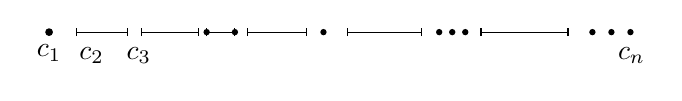
\begin{tikzpicture}[x=.69cm,y=.55cm]
\fill (0,0) circle (1.4pt);
\node[below] at (0,-.07) {$c_1$};
\foreach \a/\b in {.5/1.45,1.7/2.75,2.9/3.42,3.65/4.74,5.5/6.85,7.95/9.55}{
\draw (\a,-.09)--(\a,.09) (\a,0)--(\b,0) (\b,-.09)--(\b,.09);}
\node[below] at (.78,-.12) {$c_2$}; \node[below] at (1.65,-.12) {$c_3$};
\foreach \a in {2.9,3.42,5.05,7.18,7.42,7.66,10,10.35,10.7}{\fill (\a,0) circle (1.15pt);}
\node[below] at (10.72,-.12) {$c_n$};
\end{tikzpicture}}

\unsure{$c$|(|$C$}
% archive sheet number: 46
